\section{Reproducibility and cost}
\label{app:cost}

All model calls go through a budgeted proxy and are cached on disk by a hash of the full request, so
every number in this paper is reproducible from the released result files without re-running a model.
The compactor is \texttt{qwen3-235b-a22b-2507}; judges are \texttt{gpt-oss-120b} and
\texttt{gemma-3-27b}; a local \texttt{Qwen3-8B} supplies token log-probabilities and the write-time
pinning signal. Total inference cost for every experiment reported here, including the development
pilot and all discarded calibration runs, is given in \texttt{COST\_LOG.md}. No model was trained.

\section{Frozen protocol}
\label{app:protocol}

\texttt{FROZEN\_PROTOCOL.md} records the operating point, the control calibration, the eligibility
screen, the estimators, the clustering scheme, the decision rule and the effect-size thresholds,
together with the git commit at which they were frozen. Three amendments were made during the
development stage and are recorded there with their rationale: A1 (power and the operative smallest
effect of interest), A3 (prospective calibration of the prior-blind control) and A4 (the E-SHIFT
endpoint). No amendment was made after a confirmatory family was run.

\begin{figure}[t]
\centering
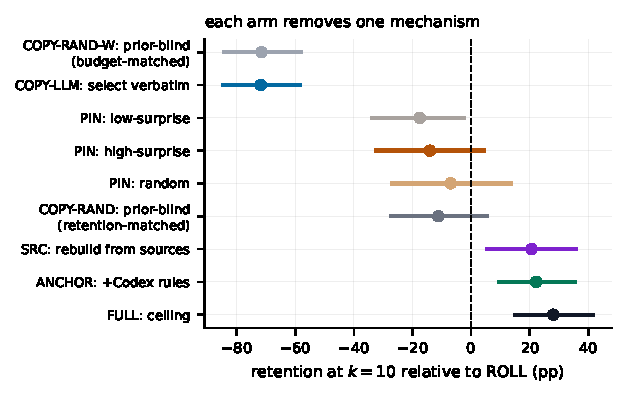
\includegraphics[width=0.92\linewidth]{figures/fig3_contrasts.pdf}
\caption{\textbf{Each arm removes one mechanism.} Retention at $k{=}10$ relative to the rolling
rewrite, with two-way crossed cluster bootstrap intervals.}
\label{fig:contrasts}
\end{figure}

\section{Robustness across models and temperature}
\label{app:robust}
The diagnostics below re-run the graded dose--response, not \textsc{E-Shift}, on smaller grids
(11 chains $\times$ 2 seeds) and score each model against the primary compactor's measured prior.
Because local 8B log-probabilities rank values only at Spearman \PThreeRho{} against that dose, a
flat slope for a different model is evidence about the portability of the stimulus set, not proof
that each model ignores its own prior.

\begin{table}[t]
\centering\small
\begin{tabular}{llcrrc}
\toprule
model & $T$ & op. & ret.\% & slope & 95\% CI \\
\midrule
Qwen3-235B (primary) & 1.0 & \textsc{o1} & 72.0 & +0.55 & [-3.0, +4.2] \\
 & 1.0 & \textsc{o4} & 92.6 & +0.23 & [-1.8, +2.5] \\
 & 1.0 & \textsc{o5} & 94.2 & -0.12 & [-2.1, +1.7] \\
 & 1.0 & \textsc{o3} & 60.8 & -0.83 & [-5.2, +3.2] \\
Qwen3-235B & 0.0 & \textsc{o1} & 71.9 & -2.11 & [-5.4, +2.0] \\
Llama-3.3-70B & 1.0 & \textsc{o1} & 11.9 & +0.19 & [-2.7, +3.3] \\
 & 1.0 & \textsc{o4} & 61.8 & -1.44 & [-6.6, +3.5] \\
 & 1.0 & \textsc{o5} & 17.4 & +0.40 & [-3.3, +5.3] \\
Qwen3-8B (local) & 1.0 & \textsc{o1} & 6.9 & -0.59 & [-2.9, +1.6] \\
 & 1.0 & \textsc{o4} & 78.2 & +1.94 & [-3.0, +7.1] \\
 & 1.0 & \textsc{o5} & 2.3 & -0.50 & [-2.6, +0.6] \\
\bottomrule
\end{tabular}
\caption{\textbf{Portability diagnostics.} Retention at $k{=}10$ and the slope of retention on measured surprise (percentage points per log-odds), with two-way crossed cluster bootstrap intervals. Every slope interval contains zero. These re-run the graded dose--response, not \textsc{e-shift}, on 11 chains $\times$ 2 seeds, and score each model against the \emph{primary} compactor's measured prior rather than its own. \textsc{o1} rewrites its own memory, \textsc{o4} rebuilds from the raw sessions, \textsc{o5} adds the Codex anti-drift rules, and \textsc{o3} is the prior-blind control (which makes no model calls and is therefore reported once). The hosted proxy caps temperature at $1.0$, so $T>1$ could not be tested.}
\label{tab:robust}
\end{table}


\section{Coder validation}
\label{app:coder}

Table~\ref{tab:coder} reports strict per-level recognition for meaning-preserving format variants and
rejection rates for decoys. Recognition is between \CoderMin{} and \CoderMax{} across levels, a
spread of \CoderSpread{}, and every unrecognised variant is routed to the blind judges rather than
mis-coded.

\section{Value-level kernel}
\label{app:kernel}
States are the measured prior rank within family ($R_1\ldots R_5$), plus \textsc{other},
\textsc{vague} and \textsc{absent}; design level names are never used, because $L_2\rightarrow L_3$
has no consistent meaning across families. The kernel is estimated from $k{=}0\rightarrow1$ on half
the trajectories with Dirichlet smoothing and applied to the held-out half, which receives the same
$p_0$ as both baselines. Deletion is close to absorbing: the regeneration rate out of \textsc{absent}
is \RegenRate{}. Held-out total-variation distances at $k{=}10$ are \KernelTVD{} for the kernel,
\KernelConstTVD{} for constant per-step survival and \KernelAbsorbTVD{} for pure absorption.

\section{Prior measurement}
\label{app:priors}

Split-half reliability of the Bradley--Terry dose is Spearman \SplitHalfRho{}
(\SplitHalfFrac{} of families at or above $0.7$). Free generation at temperature one is strongly
peaked: on average \PTwoFloor{} of five levels sit at the add-one smoothing floor, so it can report a
mode but not an ordering; it agrees with the pairwise measure on the modal level in
\PTwoModeAgree{} families. Local 8B log-probabilities correlate with the compactor's prior at only
Spearman \PThreeRho{}. The designed level ordering is the measured ordering in just
\DesignOrderAgree{} of five-level families.
